% ============================================================
%  Agentic Multimodal Systems for Medical Image Segmentation:
%  A Critical Survey of Reinforcement-Driven Approaches
%
%  Author : MD Jahid Hasan Jim
%  Course : CSE 3230 — Technical Writing & Seminar
%  Dept   : Computer Science and Engineering, KUET
%  Compile: pdfLaTeX (two passes for ToC + refs)
% ============================================================

\documentclass[12pt, a4paper]{article}

\usepackage[T1]{fontenc}
\usepackage[utf8]{inputenc}
\usepackage{mathptmx}
\usepackage{microtype}

\usepackage[a4paper, top=2.54cm, bottom=2.54cm, left=2.54cm, right=2.54cm]{geometry}

\usepackage{setspace}
\setstretch{1.15}

\usepackage{titlesec}
\titleformat{\section}      {\large\bfseries}              {\thesection.}      {0.5em}{}
\titleformat{\subsection}   {\normalsize\bfseries\itshape}  {\thesubsection}    {0.5em}{}
\titleformat{\subsubsection}{\normalsize\bfseries}          {\thesubsubsection} {0.5em}{}
\titlespacing*{\section}      {0pt}{14pt}{6pt}
\titlespacing*{\subsection}   {0pt}{10pt}{4pt}
\titlespacing*{\subsubsection}{0pt}{8pt}{3pt}

\usepackage{fancyhdr}
\pagestyle{fancy}
\fancyhf{}
\renewcommand{\headrulewidth}{0.4pt}
\fancyhead[L]{\small\itshape Agentic Systems for Medical Image Segmentation: A Survey}
\fancyhead[R]{\small\thepage}
\setlength{\headheight}{15pt}

\usepackage[colorlinks=true, linkcolor=black, citecolor=black, urlcolor=blue]{hyperref}
\usepackage{amsmath, amssymb}
\usepackage{graphicx}
\usepackage{float}
\usepackage{placeins}
\usepackage{caption}
\usepackage{subcaption}
\captionsetup{font=small, labelfont=bf, justification=centering}

\usepackage{booktabs}
\usepackage{tabularx}
\usepackage{multirow}
\usepackage{array}
\usepackage{xcolor}
\usepackage{tcolorbox}
\usepackage{pifont}

\definecolor{placeholderblue}{RGB}{46,117,182}
\definecolor{placeholderbg}{RGB}{214,228,240}
\definecolor{placeholderlight}{RGB}{235,245,251}
\definecolor{instructionred}{RGB}{192,57,43}
\definecolor{headernavy}{RGB}{31,56,100}

\newcommand{\imagePlaceholder}[5]{%
  \begin{figure}[H]\centering
    \begin{tcolorbox}[colframe=placeholderblue,colback=placeholderbg,boxrule=1.2pt,arc=2pt,left=6pt,right=6pt,top=3pt,bottom=3pt]
      \centering\bfseries\color{headernavy}[ IMAGE PLACEHOLDER \textendash{} Figure~#1 ]
    \end{tcolorbox}
    \begin{tcolorbox}[colframe=placeholderblue,colback=placeholderbg,boxrule=1.2pt,arc=0pt,top=0pt,bottom=0pt,left=6pt,right=6pt,sharp corners]
      \centering\small\itshape\color{headernavy}\textbf{Source:} #3 \quad|\quad \textbf{Reference:} #4
    \end{tcolorbox}
    \begin{tcolorbox}[colframe=placeholderblue,colback=placeholderlight,boxrule=1.2pt,arc=0pt,top=4pt,bottom=4pt,left=8pt,right=8pt,sharp corners]
      {\centering\bfseries\small\color{instructionred}\ding{72}\enspace INSTRUCTIONS TO STUDENT \enspace\ding{72}\par}
      \vspace{4pt}{\small\color{black} #5\par}\vspace{6pt}
      \begin{center}\setlength{\fboxsep}{10pt}
        \fcolorbox{gray!50}{gray!8}{\parbox[c][3.5cm][c]{0.82\textwidth}{\centering
          {\large\color{gray!70}\textbf{[ Insert figure here ]}}\\[8pt]
          {\small\color{gray!60}Screenshot or export the figure from the source PDF,\\
            upload it to Overleaf, then replace this\\
            \textbackslash imagePlaceholder command with\\
            \textbackslash includegraphics\{filename\}}}}
      \end{center}
    \end{tcolorbox}
    \vspace{4pt}\caption{#2}\label{fig:#1}
  \end{figure}}

\setlength{\parindent}{1.5em}
\setlength{\parskip}{3pt plus 1pt minus 1pt}

\usepackage{abstract}
\renewcommand{\abstractnamefont}{\large\bfseries}
\renewcommand{\abstracttextfont}{\normalfont}
\setlength{\absleftindent}{0pt}
\setlength{\absrightindent}{0pt}

\usepackage{cite}

% =============================================================
\begin{document}
% =============================================================

% ── COVER PAGE ───────────────────────────────────────────────
\begin{titlepage}
\thispagestyle{empty}\centering\vspace*{-0.8cm}
\begingroup\setstretch{1.15}


\includegraphics[width=3cm]{kuet.png}

\vspace{0.5cm}
{\normalsize\bfseries Khulna University of Engineering \& Technology\\
Department of Computer Science and Engineering}

\vspace{0.6cm}
{\small CSE 3230 : Technical Writing \& Seminar}

\vspace{0.4cm}
\noindent\rule{0.7\textwidth}{0.6pt}
\vspace{0.6cm}

{\fontsize{17}{20}\selectfont\bfseries
Agentic Multimodal Systems for Medical Image Segmentation\\[4pt]
\large A Critical Survey of Reinforcement-Driven Approaches}

\vspace{0.8cm}
{\small \textit{Prepared By}}\vspace{0.3cm}

{\normalsize\bfseries MD Jahid Hasan Jim}\vspace{0.2cm}

{\small Department of Computer Science and Engineering\\
Khulna University of Engineering \& Technology\\
Email: \texttt{jim2107054@stud.kuet.ac.bd}}

\vspace{0.8cm}
\noindent\rule{0.7\textwidth}{0.6pt}
\vspace{0.6cm}

{\small \textit{Submitted To}}\vspace{0.4cm}

{\normalsize\bfseries Dr.\ K.\ M.\ Azharul Hasan}\\
{\small Professor\\Department of Computer Science and Engineering\\
Khulna University of Engineering \& Technology}

\vspace{0.5cm}

{\normalsize\bfseries Kazi Saeed Alam}\\
{\small Assistant Professor\\Department of Computer Science and Engineering\\
Khulna University of Engineering \& Technology}

\vfill
{\small Khulna-9203, Bangladesh\\April, 2026}
\endgroup
\end{titlepage}

% ── TABLE OF CONTENTS ────────────────────────────────────────
\newpage\thispagestyle{empty}
\tableofcontents
\vspace{1cm}

% ── SOURCE TABLE ─────────────────────────────────────────────
\section*{Source Table}
\addcontentsline{toc}{section}{Source Table}
\begin{table}[H]
\centering\renewcommand{\arraystretch}{1.4}\small
\begin{tabular}{|c|p{7.5cm}|p{3.5cm}|c|}
\hline
\textbf{No.} & \textbf{Paper Title} & \textbf{Source (URL)} & \textbf{Date} \\
\hline\hline
1 & IBISAgent: Reinforcing Pixel-Level Visual Reasoning in MLLMs for Universal Biomedical Object Referring and Segmentation & \url{https://arxiv.org/abs/2601.03054} & Feb 2026 \\
\hline
2 & MEDVISTAGYM: A Scalable Training Environment for Thinking with Medical Images via Tool-Integrated Reinforcement Learning & \url{https://arxiv.org/abs/2601.07107} & Jan 2026 \\
\hline
3 & MedSAM-Agent: Empowering Interactive Medical Image Segmentation with Multi-turn Agentic Reinforcement Learning & \url{https://arxiv.org/abs/2602.03320} & Feb 2026 \\
\hline
\end{tabular}
\end{table}
\newpage

% ── ABSTRACT ─────────────────────────────────────────────────
\begin{abstract}
\noindent
The use of reinforcement learning with language models that can handle many types of data
has opened up a new way for computers to analyze medical images on their own.
Recently three systems---IBISAgent~\cite{ibisagent}, MedVistaGym and
MedVista-R1~\cite{medvistagym}, and MedSAMAgent~\cite{medsam_agent}---have
shown how computers can be trained to look at images in detail and make
clinical decisions without human help.
This review compares how these three systems work.
We look at how they are designed, how they are trained, and how they make decisions.
We also examine what they have in common and what makes them different.
These systems use a process to make decisions. They are fine-tuned in two stages before
being trained with reinforcement learning.
We find that there are still some challenges to overcome such as making these systems
faster and able to handle complex data.
We also need to find ways to give these systems information about the process
and make them better at handling new situations.
The review ends with some ideas for improvements and a look at what the next
generation of medical AI systems might be like.

\vspace{6pt}
\noindent\textbf{Keywords:} Medical Image Segmentation, Multimodal Large Language
Models, Reinforcement Learning, Agentic AI, Segment Anything Model, Interactive
Segmentation, Markov Decision Process, Tool-Integrated Reasoning.
\end{abstract}

\hrule\vspace{12pt}

% =============================================================
\section{Introduction}
\label{sec:intro}
% =============================================================

Medical image segmentation is an essential technique that possesses a primary strategic
requirement in current medical practices.
The power to detect and separate normal anatomical structures, pinpoint pathological
lesions, and measure the temporal dynamics of size and shape is central to
decision-making in oncology, radiology, cardiology, and operation scheduling.
The situation has been historical that such a task is handled through two paradigm
methods: specific functions supervised models such as U-Net~\cite{unet} and its
successors, and the interactive segmentation tools Segment Anything
Model~\cite{sam} and its medical adaptations~\cite{medsam2}.
Neither paradigm is without its drawbacks, which limit their usefulness at a larger
scale.
Supervised models dominate the scores in narrow ranges of the datasets they train on
and are not relevant to the other situations or the standards they require.
The interactive types of MedSAM~\cite{medsam2} on the other hand are the opposite for
they solve the distribution shift problem mainly due to their method of
prompt-conditioned inference.
Nevertheless, they transfer the cognitive load to the clinicians who are required to
provide a number of bounding boxes or click prompts for every single case---this is
not feasible in a large number of patients.

The rise of MLLMs has demonstrated a third way to be undertaken: machines that can
comprehend the human language notes, deduce the visible information, and take
actions---they displace the human prompter with the independent reasoning agent.
Such outstanding work as LISA~\cite{lisa} has shown that a single \texttt{<SEG>}
token which is included in the MLLM output stream can be decoded by an external pixel
decoder.
The idea was elegant but carried a structural cost: inserting an implicit task token
shifts the model's native language representation space, impairing open-ended reasoning
and cross-domain generalisation~\cite{ibisagent}.
A subtler limitation is that all of these approaches treat segmentation as a single
forward pass---one look at the image, one prediction, done.
Human annotators do not work that way; they place an initial mark, check the result,
correct mistakes, and iterate until satisfied.

Three groups, working independently, published papers in early 2026 that all converge
on the same alternative: reformulate segmentation as a multi-step agent-environment
interaction loop and use RL to train the agent.
IBISAgent~\cite{ibisagent} generates text-encoded click commands, sends them to
MedSAM2, observes the updated mask, and refines its plan before taking the next click.
MedVistaGym and MedVista-R1~\cite{medvistagym} build a Gym-style environment containing
fifteen visual and biomedical knowledge tools and train an InternVL3-based agent to
select and invoke the right tool at the right moment.
MedSAM-Agent~\cite{medsam_agent} expands the action vocabulary to include bounding
boxes as well as click points, and introduces a process-aware reward that penalises
both overshooting a good segmentation and taking needlessly many steps.

Although the three AI systems all aim at automating medical image segmentation, they
involve different action-space formulations, reward mechanisms, scales of required
training data, and evaluation procedures.
The results reported with respect to these approaches cannot be taken as an indication
of what one can expect with the others. Comparing and contrasting these three AI
systems offers a timely opportunity to raise awareness of the practical challenges in
building agentic segmentation systems and the associated limitations of current
methodologies for designing and evaluating such systems.

\begin{figure}[H]
  \centering
  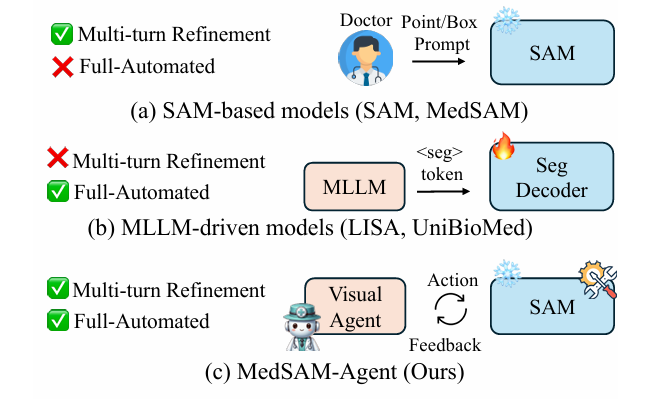
\includegraphics[width=\linewidth]{fig1.png}
  \caption{A schematic comparison of three paradigms for medical image segmentation.
   (a)~SAM-derived interactive models requiring manual prompts for every case.
   (b)~MLLM-driven models using implicit \texttt{<SEG>} tokens decoded by an external
   pixel head. (c)~The autonomous agentic paradigm, illustrated by MedSAM-Agent, where
   the agent refines the mask iteratively through a feedback loop without human
   involvement. Adapted from Liu et al.~\cite{medsam_agent}.}
  \label{fig:1}
\end{figure}

The rest of this review is organized as follows.
We provide an overview of the three systems with a focus on the assumptions, goals,
and organization in Section~\ref{sec:background}.
Section~\ref{sec:methodology} presents in-depth analyses of how model human cognition
has been incorporated in each system.
This is followed by a side-by-side comparison in Section~\ref{sec:discussion}.
We then synthesize similarities and differences between the three in
Section~\ref{sec:synthesis}.
After this we identify key issues and draw implications.
A discussion on the relations between modeling and supporting designers and on MLGOs
in particular is also provided.

% =============================================================
\section{Background and Related Work}
\label{sec:background}
% =============================================================

\subsection{Medical Image Segmentation: A Brief History}

The course of research on medical image segmentation over the last ten years has been
a battlefield between specificity and generality.
The methods based on fully convolutional networks like U-Net~\cite{unet} not only
achieved good results inside one dataset, but they also needed retraining for each new
task.
The nnU-Net~\cite{nnunet} which is an innovative model had a self a training pipeline
for details but it still included the basic rule of task-specific parameter settings.
Transformer-based structures have added the receptive field and improved the concept of
spatial dependencies which are of long range, yet, the core paradigm is still the same.
The release of the SAM~\cite{sam} was a bucket of fresh thought as it was not a succor
but a prognosis, the agnostic segmentation basis.
SAM has points, bounding boxes, or masks as the prompts that it accepts and
high-quality segmentation is produced across many different natural image domains.
MedSAM~\cite{medsam2} was this type of adaptation applied to biomedical imaging by
fine-tuning on large-scale annotated medical datasets, which showed a remarkable boom
in performance compared to zero-shot SAM.
MedSAM2~\cite{medsam2} was the first in history to add the stereoscopic and dynamic
video technology to the scope of the approach.
But to make use of these models, experts should provide prompts in the inference time.

\subsection{Connecting MLLMs to Pixel-Level Prediction}

In this paper we present a method to enhance Multiple Label Learning Models (MLLMs)
for pixel-wise visual classification.
In natural language inference, current models are evaluated on accuracy.
In this paper, we examine an alternate objective for the challenging task: we introduce
and evaluate reasoning segmentation for natural language inference.
With input sentences parsed into separate, individuable steps of reasoning, a model
must first learn to segment a sentence into distinct reasoned arguments before learning
to select the correct response to a given inference task.
We systematically examine models presented with all possible partitions of input
sentences and find that some models can learn to select optimal partitions with
state-of-the-art accuracy.
In this paper, we explore the task of producing segmentation masks for natural language
input.
We present an approach which processes complex natural language input and directly
generates a proper segmentation mask as output.
The approach learns a special \texttt{<SEG>} embedding, and then it uses a SAM-like
pixel decoder to decode the hidden states for this embedding.
Several approaches extended this idea to medicine.
MedPLIB~\cite{medplib}: in order to get insight on groups of pixels LISA was extended
to also get insight on the single pixel level, with applications in biomedicine.
UniBiomed~\cite{unibiomed} extended the universal biomedical foundation model to also
address the task of grounded image interpretation.
Citrus-V~\cite{citrusv} advanced unified medical grounding for clinical reasoning.
In this paper we reveal two basic structural limitations of current LISA-style systems.
Implicit tokens in language model output shifts the language generation distribution to
force the model to be less open-ended in capability than it would be otherwise.

\subsection{Tool-Augmented and Agentic Reasoning in Medicine}

The idea of augmenting language models with callable tools has a long history in NLP,
but its application to medical visual reasoning took off partly in response to
DeepSeek-R1~\cite{deepseekr1}, which showed that RL from verifiable rewards could
dramatically improve structured reasoning.
MMedAgent~\cite{mmedagent} trained a medical MLLM to invoke specialist tools through
instruction tuning, and VILA-M3~\cite{vilam3} triggered expert perception modules, but
both treated tool use as a fixed, single-step function call.

This two-part e-book continues the theme started in Beyond Visual Acuity and explores
the topic of tools---what they can do for medical vision, and the benefits of tool use
by clinicians.
When reasoning, one needs to learn how to use tools, and also how to employ disciplined
interaction policies.
All three systems reviewed here use RL to train that kind of multi-turn orchestration---
the central technical contribution shared by IBISAgent~\cite{ibisagent},
MedVistaGym/MedVista-R1~\cite{medvistagym}, and MedSAM-Agent~\cite{medsam_agent}.

% =============================================================
\section{Methodology}
\label{sec:methodology}
% =============================================================

\subsection{IBISAgent: Iterative Biomedical Interactive Segmentation Agent}
\label{sec:ibis}

\subsubsection{Motivation and Core Idea}

The team of researchers from the Zhejiang University, and the Shanghai AI Lab developed
IBISAgent~\cite{ibisagent}, to solve the structural issues that exist with current
Medical Language Models for Masked Language Modeling (MMLM): explicit segmentation
tokens that damage the language representation space and restrict models to perform
inference one time to prevent iterative masking refinement.
The key idea behind developing IBISAgent is to treat masked language modeling as a
Multi-Step Markov Decision Process (MDP) where the MLM generates text-based click
commands, calls an interactive segmentation tool (MedSAM2~\cite{medsam2}) and updates
the action plan according to the resulting mask observation.
This way the original space of text output of the MLM remains intact.
Instead of emitting a token, the model produces action strings that contain the target
class, the click polarity ($+/-$) and the normalized 2D coordinates.
The process continues until the model determines that the mask is acceptable; at this
point it terminates and produces a natural language answer.

\subsubsection{Architecture and Rollout Mechanics}

In its formal definition, the interaction trajectory $\mathcal{P}$ of IBISAgent is
defined as $\mathcal{P} = \{(r_t, a_t, o_t)\}_{t=1}^{T}$, where $r_t$ is the
reasoning at step $t$, $a_t$ is the click action, and $o_t$ is the observation of
segmentation---an image that overlays the current mask on top of the original image in
a semi-transparent way.
Such composite observations are then encoded by the vision encoder at every step,
making it possible to perceive the boundary of the current mask and the underlying
anatomy simultaneously.
The thought-action-observation cycle continues until an explicit end token is generated
or a maximum context length is achieved.
Actions consist of three parts per click: Target (name of segmentation classes),
Attribute ($\alpha \in \{+1,-1\}$), and Coordinate\_2d ($(x,y) \in [0,1]^2$).
Observation $o_0$ is set to be an empty mask, while $o_T$ corresponds to the optimal
target mask.

\begin{figure}[H]
  \centering
  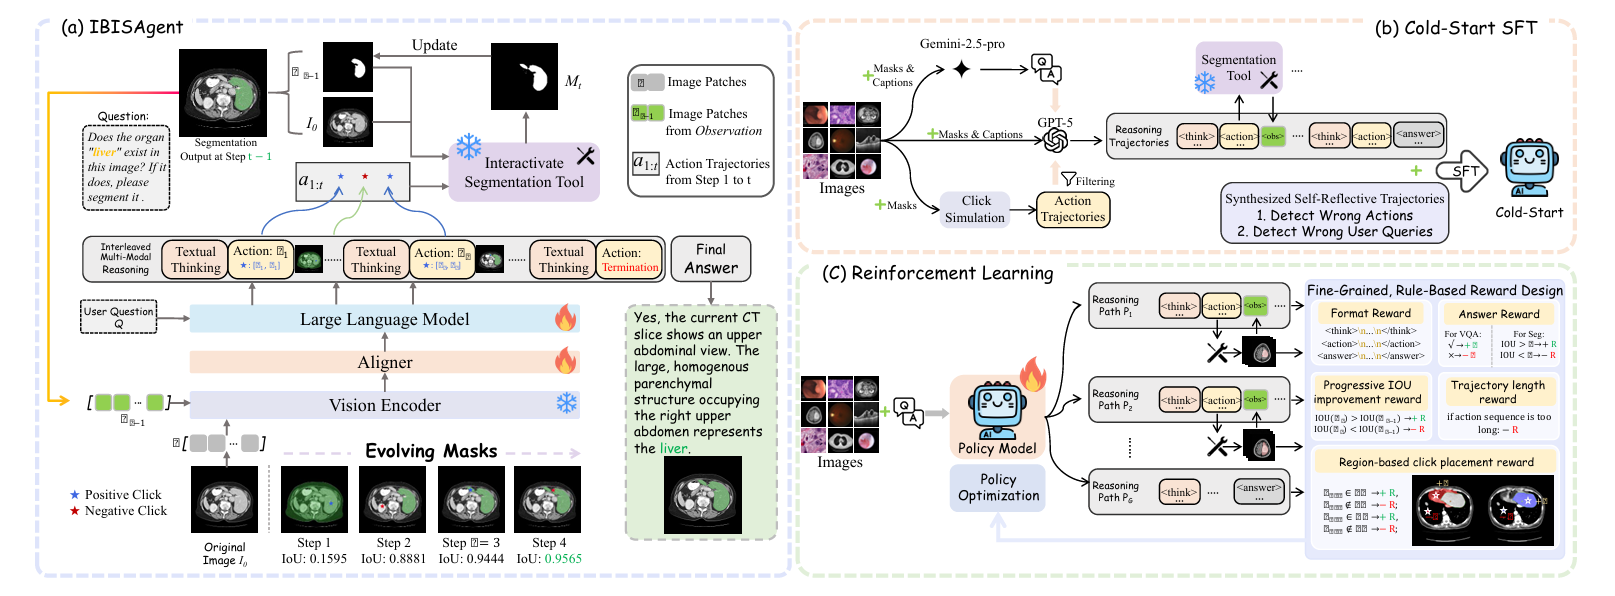
\includegraphics[width=\linewidth]{fig2.png}
  \caption{Overview of the IBISAgent framework.
   (a)~The iterative thought-action-observation loop: the agent reasons, emits a click
   action, and receives an updated composite image at each step.
   (b)~The cold-start SFT pipeline, where Gemini-2.5-Pro generates question-answer
   pairs and GPT-5 synthesises step-by-step reasoning traces via a Teacher-Student
   strategy.
   (c)~The RL stage with the five-component reward signal.
   Adapted from Jiang et al.~\cite{ibisagent}.}
  \label{fig:2}
\end{figure}

\subsubsection{Building the Training Data}

The major challenge in building the IBISAgent was the unavailability of any trajectory
for click steps, which can be publicly accessible.
To address this constraint, the authors utilized an automatic click simulation technique
that was applied on BioMedParseData dataset~\cite{biomedparse} which contains 3.4
million clicks with an image-mask-label triplet for 82 biomedical object classes over 9
imaging modalities.
With the help of the ground-truth mask $M_{\text{gt}}$ and the predicted mask $M_t$,
the simulator is capable of locating the FP and FN areas, performing a Euclidean
distance transform operation, and clicking at the center of the largest error
area---an approach borrowed from previous literature in interactive
segmentation~\cite{deepinteractive}.

Different question-answer pairs were formed using
Gemini-2.5-Pro~\cite{gemini25}.
Thereafter, GPT-5~\cite{gpt5} was used to generate the trajectory in the form of
reasoning via Teacher-Student pipeline for every click without any knowledge of
ground-truth labels.

In addition to rotation, color and brightness augmentation and mirroring, we also
generate trajectories where the virtual view-point reflects off the surface of two
walls in the same room.
This results in a large number of distinct viewing positions.
Errors and situations where error correction happens while the error is being made,
i.e., the agent recognises it is making a mistake and undoes the wrong action.
And user-inconsistency correction (where the initial mask provided by the user fails
to match).
After quality filtering, $\mathcal{D}_\text{cold}$ contains
456,000 samples with a mean trajectory length of 8.69 steps and overall mean IoU
of 94.27.

\begin{figure}[H]
  \centering
  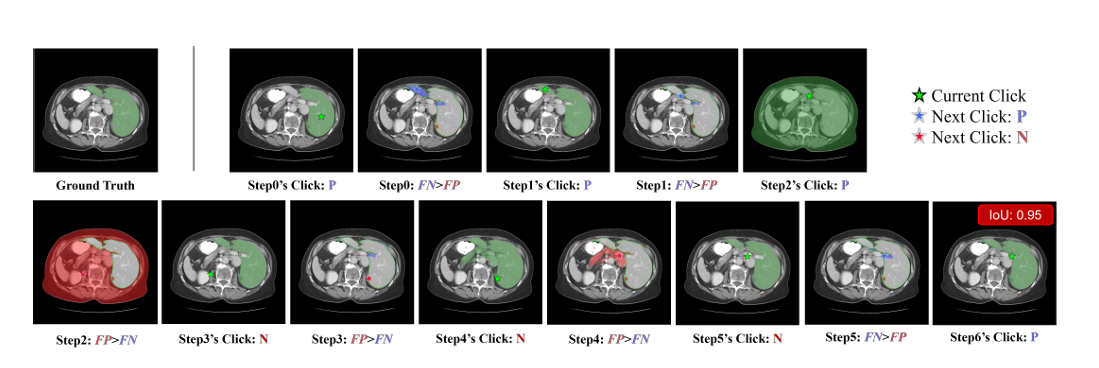
\includegraphics[width=\linewidth]{fig3.png}
  \caption{Automated trajectory generation for liver segmentation in IBISAgent.
   At each step, positive clicks (blue) are placed in under-segmented (false-negative)
   regions and negative clicks (red) in over-segmented (false-positive) regions.
   IoU rises from 0 to roughly 0.95 across seven interactions.
   Adapted from Jiang et al.~\cite{ibisagent}.}
  \label{fig:3}
\end{figure}

\subsubsection{Two-Stage Training}

The training procedure for IBISAgent consists of two phases.
First, cold start supervised fine-tuning (SFT) trains the network to output
syntactically correct sequences of actions, to provide anatomically reasonable
reasoning, and to display self-repair behavior.
The loss function for SFT training is a classic negative log-likelihood loss applied to
reasoning and action tokens.

Stage two applies GRPO~\cite{deepseekr1} on $\mathcal{D}_\text{rl}$ (888K VQA
samples mixing pixel-level and general medical VQA).
The reward is a normalised average of five components:
\begin{enumerate}
  \item \textbf{Format reward} $S_\text{format}$: checks required tokens appear in
        correct order and \texttt{<action>} fields are parseable;
  \item \textbf{Final-answer reward} $S_\text{ans}$: piecewise IoU reward for
        segmentation; exact match for VQA;
  \item \textbf{Region-based click placement reward} $S_\text{click}$: positive clicks
        must land in FN regions, negative clicks in FP regions;
  \item \textbf{Progressive improvement reward}
        $S_\text{pseg} = \mathbb{1}(\Delta\text{IoU}_t > 0)$: each step must improve
        the mask;
  \item \textbf{Trajectory length reward} $S_\text{len}$: growing penalty for sequences
        exceeding the optimal length $T_\text{opt}$.
\end{enumerate}
Final reward: $S = \frac{1}{5}(S_\text{ans}+S_\text{format}+S_\text{click}+S_\text{pseg}+S_\text{len})$.

\subsubsection{Experimental Results}

IBISAgent is evaluated on three benchmarks: a 9K in-domain test set from
BioMedParseData, the out-of-domain MeCOVQA-G+ benchmark~\cite{medplib} (3,157 pairs
across five modalities), and a private held-out dataset from three medical centres
with 1K CT, MRI, and histopathology images across seven cancer types.
On the in-domain split: IoU~=~85.58\%, DSC~=~92.21\%, F1~=~96.39\%.
The nearest competitor, UniBiomed~\cite{unibiomed}, scores IoU~=~50.74\%, a gap of
roughly 35 percentage points.
On MeCOVQA-G+: 80.63\% vs 46.54\% for Citrus-V~\cite{citrusv}.

\begin{figure}[H]
  \centering
  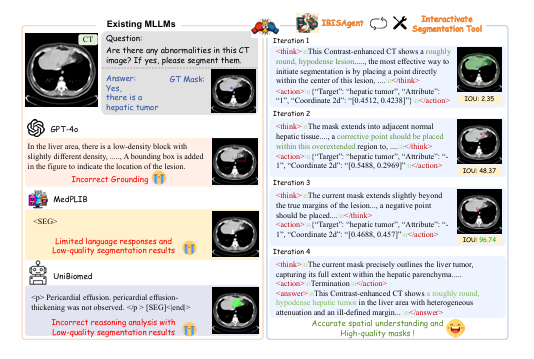
\includegraphics[width=\linewidth]{fig4.png}
  \caption{Qualitative comparison on a hepatic tumour segmentation case.
   GPT-4o misidentifies the lesion location; MedPLIB outputs only a \texttt{<SEG>}
   token with no clinical reasoning; UniBiomed hallucinates a pericardial effusion
   absent from the image.
   IBISAgent refines the mask over four steps, reaching IoU~=~96.74\% alongside
   coherent clinical text. Adapted from Jiang et al.~\cite{ibisagent}.}
  \label{fig:4}
\end{figure}

The ablation studies clearly show that reinforcement learning is the main driver behind
the performance boost.
At the same time, each of the five reward components plays its own role, independently
contributing to better segmentation quality as well as more efficient interactions.

% ──────────────────────────────────────────────────
\subsection{MedVistaGym and MedVista-R1: Tool-Integrated Reasoning}
\label{sec:medvista}
% ──────────────────────────────────────────────────

\subsubsection{Motivation and Core Idea}

In this regard, the MedVistaGym paradigm~\cite{medvistagym}, conceived by researchers
from Virginia Tech, UT Southwestern Medical Center, Georgia Institute of Technology,
and Cisco, focuses on a different but related problem: allowing VLMs to reason over
medical images by dynamically selecting and invoking external tools, rather than being
limited to a predetermined segmentation backend.
Tool access alone is not enough---as the ablations demonstrate, giving a strong
baseline model tools without structured training actually \emph{hurts} performance.
What the agent needs is an RL regime that teaches it \emph{when} to invoke a tool,
\emph{which} one to pick, and how to synthesise the returned observation into a revised
reasoning chain.

To operationalise this, the team built MEDVISTAGYM: a Gym-style executable environment
wrapping fifteen tools under a unified API, grouped into four families: Resolution and
Region Refinement (e.g., 4KAgent), Medical Localisation and Segmentation (e.g.,
GroundingDINO, SAM2, BioMedParse, MedSAM2), Medical Visual Understanding
(e.g., BiomedCLIP), and External Knowledge Retrieval (e.g., PubMed, DrugBank).

\subsubsection{Problem Formulation}

MEDVISTAGYM formalises the problem as a Partially Observable MDP.
An interaction trajectory $U = (g_0, a_0, \ldots, g_T, \hat{y})$ records reasoning
steps $g_t$, tool invocations $a_t$, and the final answer $\hat{y}$ after $T$ steps.
The fixed output format---
\texttt{<think>}\,$\ldots$\,\texttt{</think>}
\texttt{<tool\_call>}\,$\ldots$\,\texttt{</tool\_call>}
\texttt{<think>}\,$\ldots$\,\texttt{</think>}
\texttt{<answer>}\,$\ldots$\,\texttt{</answer>}---
basically makes the agent slow down and think things through properly.
It has to reason first before calling any tool, then pause and rethink after seeing the
result, and only then give the final answer.
This flow keeps the process more thoughtful and structured, instead of letting the
model jump straight to a conclusion without reflecting on what just happened.

\subsubsection{Training Data and Trajectory Generation}

The training data of MedVista-R1 is generated using datasets like
PathVQA~\cite{pathvqa}, SLAKE~\cite{slake}, and VQA-RAD~\cite{vqarad}.
During live simulation in the environment called MEDVISTAGYM, GPT-5~\cite{gpt5} is
applied to produce reasoning trajectories along with invoking tools.
The final trajectories selected are the ones that produce the right answer to the
question based on the ground truth.
This is followed by applying the GPT-5~\cite{gpt5} model to assign an ordinal score
of 1 to 4.

\subsubsection{Training and Reward Design}

MedVista-R1 is initialised from InternVL3 (2B and 8B).
Stage one uses behavioural cloning to establish reliable tool invocation syntax.
Stage two applies GRPO within MEDVISTAGYM with a three-component reward:
\begin{enumerate}
  \item \textbf{Format reward} $R_\text{format}$: all required special tokens present
        in the correct order;
  \item \textbf{Accuracy reward} $R_\text{acc}=\mathbb{1}[\hat{y}=y]$: binary
        predicted-vs-ground-truth match;
  \item \textbf{Conditional tool-use reward} $R_\text{tool}$: granted only when the
        trajectory invokes at least one tool \emph{and} produces the correct answer.
\end{enumerate}
Total: $R(U)=R_\text{format}(U)+R_\text{acc}(U)+R_\text{tool}(U)$.
The conditional design of $R_\text{tool}$ teaches the agent to understand \emph{when}
tools genuinely help, rather than calling them indiscriminately.

\subsubsection{Experimental Results}

MedVista-R1-8B reaches 73.70\% on the in-domain average and 63.09\% overall.
The vanilla InternVL3-8B backbone scores 61.36\% and 54.66\% respectively.
Most revealing: InternVL3-8B with tool access but no RL scores only 38.88\%---lower
even than the no-tool baseline.
This is the clearest demonstration in any of the three papers that tool access is not
plug-and-play; without the right training, tools introduce confusion rather than
clarity.

\begin{figure}[H]
  \centering
  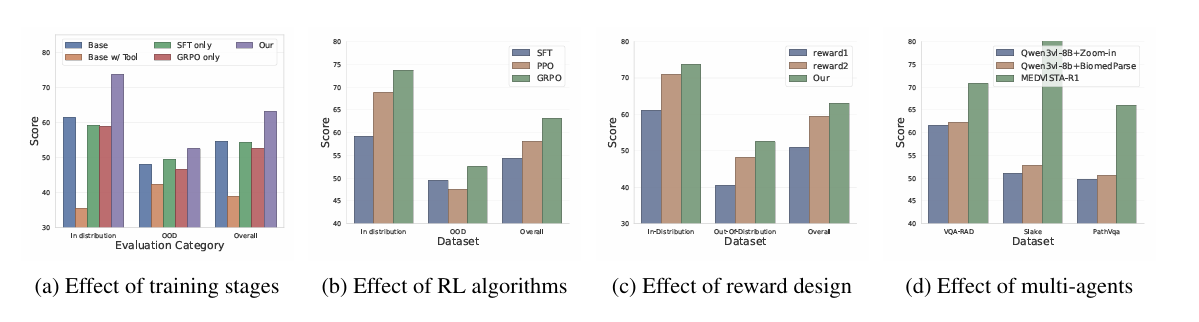
\includegraphics[width=\linewidth]{fig6.png}
  \caption{Ablation results for MedVista-R1 across four experimental dimensions:
   (a)~effect of different training stages, (b)~comparison of RL algorithms
   (SFT, PPO, GRPO), (c)~impact of reward design choices, and (d)~multi-agent
   workflow alternatives. Adapted from Lu et al.~\cite{medvistagym}.}
  \label{fig:6}
\end{figure}

% ──────────────────────────────────────────────────
\subsection{MedSAM-Agent: Multi-turn Agentic RL for Interactive Segmentation}
\label{sec:medsam}
% ──────────────────────────────────────────────────

\subsubsection{Motivation and Core Idea}

Liu et al.~\cite{medsam_agent} share with IBISAgent the goal of autonomous iterative
segmentation, but address two limitations in prior work.
First, a pure point-click space lacks flexibility for morphologically heterogeneous
structures: large organs can be localised far more efficiently with a bounding box.
Second, existing RLVR frameworks are outcome-focused---they reward final segmentation
quality but ignore whether the agent took redundant steps, which matters for both
training convergence and clinical deployment.

\begin{figure}[H]
  \centering
  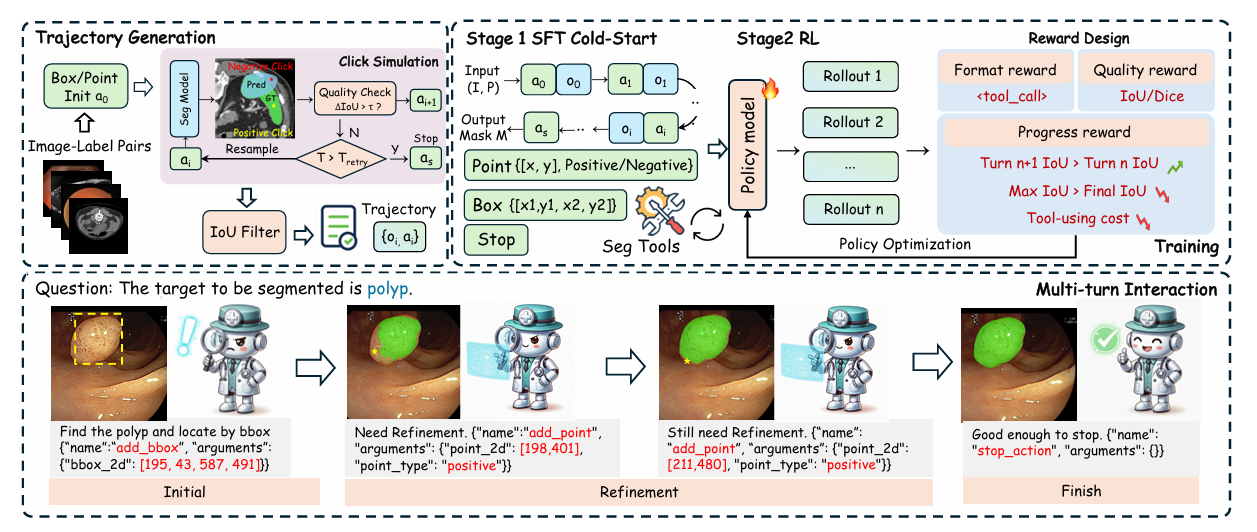
\includegraphics[width=\linewidth]{fig7.png}
  \caption{Overview of the MedSAM-Agent framework.
   The upper portion shows the hybrid trajectory generation strategy
   (Box-to-Point and Sequential-Click workflows) with progress-constrained sampling
   and IoU-based filtering.
   The lower portion shows the two-stage training pipeline (SFT cold-start and
   GRPO-based RL) and the five-component process-aware reward design.
   A qualitative polyp segmentation example illustrates multi-turn refinement.
   Adapted from Liu et al.~\cite{medsam_agent}.}
  \label{fig:7}
\end{figure}

\subsubsection{Action Space and Observation}

MedSAM-Agent's action vocabulary has three primitives.
\texttt{add\_bbox} submits $[x_1,y_1,x_2,y_2]$ for global spatial context;
\texttt{add\_point} submits $[x,y]$ with polarity $\alpha\in\{+1,-1\}$ for local
refinement; \texttt{stop\_action} terminates the loop when the mask is satisfactory.
The observation $o_t$ represents the updated predicted mask $M_t$, which is generated
by the segmentation backend---either MedSAM2~\cite{medsam2} or
IMISNet~\cite{imisnet}.
Instead of introducing a separate \texttt{<think>} token during reinforcement learning,
the model is intentionally designed without it.
This forces the system to embed its spatial reasoning directly into the action
generation process, rather than relying on an explicit intermediate reasoning step.
As a result, decision-making becomes more tightly coupled with the actual prediction
behavior, leading to a more efficient and integrated learning mechanism.

\subsubsection{Hybrid Trajectory Generation}

Two parallel generation workflows are implemented.
In the Box-to-Point workflow, $a_0$ is a bounding box from the ground-truth mask
boundary with jitter $\epsilon\sim U(-\delta,\delta)$ to simulate human imprecision.
In the Sequential-Click workflow, $a_0$ is a centroid click.
All subsequent steps use the same error-driven mechanism: compute FN and FP regions,
apply a distance transform, and sample the next click from the centroid of the larger
error region.

A progress-constrained mechanism requires $\Delta\text{IoU}\geq\tau$ (default 0.04)
per step; the simulator resamples up to $N=5$ positions if the constraint is not met.
After global IoU filtering, the SFT dataset contains 449K--519K monotonically
improving trajectories.

\subsubsection{Process-Aware Reward Design}

\[
  R_\text{total} = w_1\cdot R_\text{fmt}
    + w_2\cdot\text{clip}\!\left(R_\text{qual}
      +\lambda_1 R_\text{imp}-\lambda_2 R_\text{over}-\lambda_3 R_\text{cost},\;0,\;1\right)
\]
\begin{itemize}
  \item $R_\text{fmt}$: 0.5 points each for a valid tool invocation and stop action;
  \item $R_\text{qual}=w_\text{iou}\cdot\text{IoU}_\text{final}
        +w_\text{dice}\cdot\text{Dice}_\text{final}$: quality on the final mask;
  \item $R_\text{imp}=\sum_{t=1}^{N-1}\max(0,\text{IoU}_t-\text{IoU}_{t-1})$:
        Progressive Improvement Bonus;
  \item $R_\text{over}=\text{IoU}_\text{max}-\text{IoU}_\text{final}$: Overshoot
        Penalty for quality regression after the peak;
  \item $R_\text{cost}$: linear Tool-Cost Penalty proportional to sequence length.
\end{itemize}
The Overshoot Penalty, absent from the other two papers, teaches an explicit stopping
policy by penalising any further interaction after peak quality.

\subsubsection{Experimental Results}

MedSAM-Agent is evaluated across 21 datasets covering six modalities.
With MedSAM2, it achieves overall Dice~=~0.794 and IoU~=~0.705, versus 0.776 Dice
for UniBiomed, 0.482 for Citrus-V, and 0.353 for Seg-R1~\cite{segr1}.
Mean interaction turns: 2.11 with full SFT+RL versus 2.35 with SFT only, confirming
that process-aware rewards genuinely reduce unnecessary steps.

\begin{figure}[H]
  \centering
  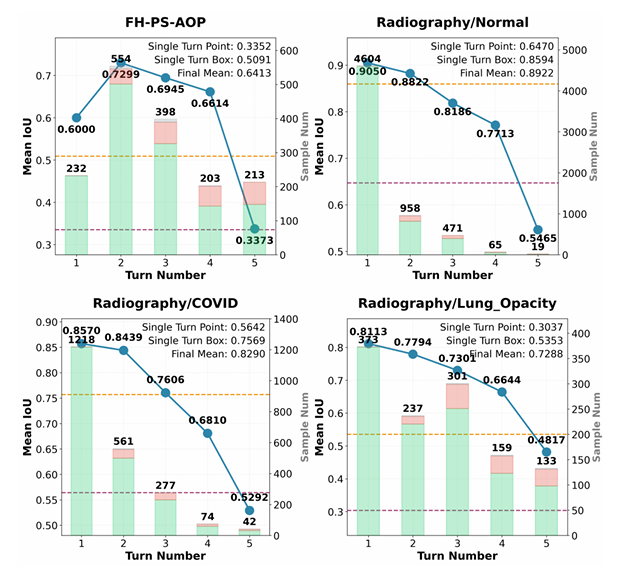
\includegraphics[width=0.80\linewidth]{fig8.png}
  \caption{Multi-turn interaction analysis for MedSAM-Agent across four datasets.
   The blue line tracks mean IoU per turn; horizontal lines mark single-turn
   ground-truth baselines (box and centroid click).
   The stacked bars show the fraction of samples with improving (green), declining
   (red), and unchanged (grey) IoU at each turn.
   Adapted from Liu et al.~\cite{medsam_agent}.}
  \label{fig:8}
\end{figure}

Zero-shot tool generalisation experiments also show that an agent trained with MedSAM2
achieves competitive performance when switched to IMISNet or SAM2 at inference, with
IoU drops under 0.02 in most settings.

% =============================================================
\section{Discussion}
\label{sec:discussion}
% =============================================================

\subsection{Summary Comparison}

Table~\ref{tab:comparison} places the three reviewed systems alongside key baselines.

\begin{table}[htbp]
\centering
\caption{How the three main systems compare with representative baseline approaches.
Methods shown in bold are the focus of this review. Where data is unavailable or
irrelevant, we use ``--''.}
\label{tab:comparison}
\renewcommand{\arraystretch}{1.25}
\footnotesize
\begin{tabular}{@{}p{2.8cm}p{2.2cm}p{1.7cm}p{1.9cm}p{1.5cm}p{1.4cm}c@{}}
\toprule
\textbf{Method} & \textbf{Action Space} & \textbf{Interaction}
& \textbf{Training} & \textbf{In-Domain} & \textbf{OOD} & \textbf{Params} \\
\midrule
\multicolumn{7}{@{}l}{\textit{The three agent-based systems with iterative refinement}} \\[2pt]
\textbf{IBISAgent}~\cite{ibisagent}     & Click points   & MDP   & SFT+GRPO & 85.58\% IoU  & 72.09\% IoU  & 7B \\
\textbf{MedSAM-Agent}~\cite{medsam_agent} & Box+points   & MDP   & SFT+GRPO & 0.794 Dice   & 0.720 Dice   & 8B \\
\textbf{MedVistaGym}~\cite{medvistagym} & Tool API calls & POMDP & SFT+GRPO & 81.36\% Acc. & 56.43\% Acc. & 8B \\
\midrule
\multicolumn{7}{@{}l}{\textit{Baselines (implicit-token, single-pass)}} \\[2pt]
LISA~\cite{lisa}           & \texttt{<SEG>} token & Single-pass & SFT  & Low         & Very low    & 7B \\
UniBiomed~\cite{unibiomed} & \texttt{<SEG>} token & Single-pass & SFT  & 0.776 Dice  & 0.317 Dice  & 1B \\
\midrule
\multicolumn{7}{@{}l}{\textit{Baselines (interactive, single-turn)}} \\[2pt]
MedSAM2~\cite{medsam2}    & Bounding box  & Single-turn & None & 82.07\% IoU & 71.30\% IoU & --  \\
MMedAgent~\cite{mmedagent} & Tool calls    & Single-turn & SFT  & 36.13\% IoU & 26.54\% IoU & 7B  \\
\bottomrule
\end{tabular}
\end{table}

\FloatBarrier

\subsection{Dataset Scale and Modality Coverage}

Table~\ref{tab:datasets} summarises dataset characteristics.

\begin{table}[htbp]
\centering
\caption{Training data characteristics across the three systems.
Note: SFT refers to the supervised fine-tuning stage, while RL indicates the
reinforcement learning phase.}
\label{tab:datasets}
\renewcommand{\arraystretch}{1.25}
\footnotesize
\begin{tabular}{@{}p{2.8cm}p{4cm}p{1.9cm}cp{3cm}@{}}
\toprule
\textbf{System} & \textbf{Primary Dataset(s)} & \textbf{Image Scale}
& \textbf{Modalities} & \textbf{Training Samples} \\
\midrule
IBISAgent~\cite{ibisagent}
  & BioMedParseData~\cite{biomedparse} & 3.4M images & 9 & 456K SFT + 888K RL \\
MedSAM-Agent~\cite{medsam_agent}
  & 21 open-source datasets & 419K images & 6 & 449K SFT + 9K RL \\
MedVistaGym~\cite{medvistagym}
  & PathVQA, SLAKE, VQA-RAD + OOD & $\approx$10K QA pairs & Mixed & $\approx$10.5K SFT \\
\bottomrule
\end{tabular}
\end{table}

IBISAgent uses the biggest training set in terms of the number of raw images, with
456,000 images from a collection of 3.4 million used for SFT, along with 888,000 images
for RL, thus emphasizing the data-oriented nature of click trajectory-based learning
models.
MedSAM-Agent is of a similar magnitude in terms of SFT and uses carefully selected
9,000 images for RL.
In turn, MedVistaGym/MedVista-R1 uses a relatively small dataset, yet makes up for it
with the diversity of reasoning trajectories for multiple tools.

\subsection{Action Space Comparison}

The most significant difference between the three approaches is in the definition of
the agent's action space.
IBISAgent only allows actions in the form of normalized point-click interactions paired
with a stop signal.
Such a simple interaction model allows for precise spatial reasoning but forces the
agent to start every segmentation process from an empty mask, which is sometimes
inefficient for large anatomically distinct structures.

MedSAM-Agent overcomes this drawback by adding bounding box initialization.
According to~\cite{medsam_agent}, the use of bounding boxes significantly decreases
the average number of actions per trajectory from 2.94 to 2.06 and increases the
intersection-over-union value of the final result from 0.623 to 0.649, where the
hybrid method achieves 0.686.

MedVistaGym/MedVista-R1 takes a completely different approach to defining the action
space since it uses high-level JSON invocations of tools instead of low-level
point-click interactions.

\subsection{Reward Function Design}

IBISAgent's five-component reward is the most elaborate, with the region-based click
placement reward $S_\text{click}$ being particularly important: it prevents the agent
from finding degenerate policies where accidentally well-placed clicks produce correct
masks by coincidence.
MedSAM-Agent's Overshoot Penalty is unique---it provides an explicit stopping criterion
beyond the softer trajectory length penalty in IBISAgent.
MedVistaGym's reward is the sparsest, but the conditional design of $R_\text{tool}$
cleverly prevents learning to call tools without actually using their outputs.

\begin{figure}[H]
  \centering
  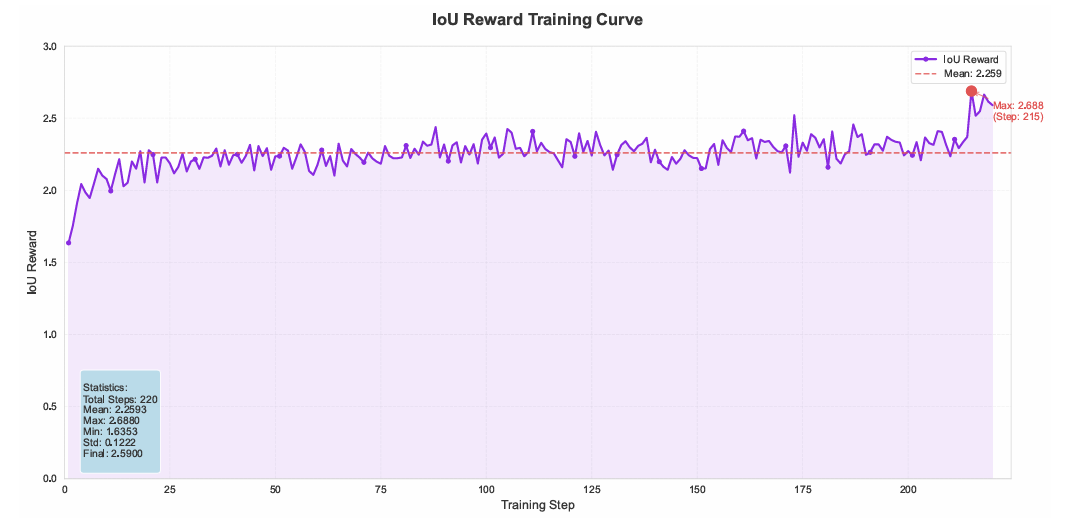
\includegraphics[width=0.92\linewidth]{fig9.png}
  \caption{IoU reward training curve for IBISAgent across 220 RL steps
   (mean~=~2.26, peak~=~2.69 at step~215).
   The curve rises steadily with no signs of reward hacking or policy collapse,
   confirming stable training throughout.
   Adapted from Jiang et al.~\cite{ibisagent}.}
  \label{fig:9}
\end{figure}

\subsection{Generalisation to Unseen Distributions}

IBISAgent's held-out in-house dataset---from three medical centres covering seven
cancer types not seen during training---is the most demanding test of any of the three
papers.
The 72.09\% IoU achieved there, versus under 36\% for all LISA-style baselines, is a
compelling result.
MedSAM-Agent's cross-tool experiments show the learned interaction policy is at least
partly tool-agnostic, which matters because a clinical site may not have the specific
backend used in training.
MedVistaGym achieves 52.48\% OOD accuracy with no OOD samples in training.

\subsection{Computational Overhead}

IBISAgent reports 28.70 seconds per sample on an A100 GPU, roughly three times the
cost of single-pass baselines.
MedSAM-Agent's process rewards keep the mean trajectory at 2.11 turns, limiting
overhead.
MedVistaGym caps tool calls at six per query and finds that longer reasoning
trajectories correlate with accuracy, pointing to a depth-versus-cost trade-off.

% =============================================================
\section{Integrative Synthesis and Future Frontiers}
\label{sec:synthesis}
% =============================================================

\subsection{What All Three Systems Agree On}

Several design choices appear in all three papers despite the groups working
independently---suggesting they reflect genuine insights rather than preferences.

Two-stage training (SFT cold-start followed by RL) substantially outperforms either
stage alone in every ablation across all three papers.
The SFT stage provides the syntactic and semantic scaffolding without which RL
exploration is too unstable to converge on good policies.

All three systems also re-encode the evolving visual state at each step rather than
relying on a fixed embedding from the initial forward pass.
The shared intuition is that pixel-level reasoning cannot be done from a single static
representation when the task involves iterative boundary refinement.

Finally, all three papers show that tool access without structured policy training is
neutral or harmful.
Simply exposing a capable VLM to medical tools will not produce good results---the
interaction policy must be explicitly trained through RL.

\subsection{Open Challenges}

A move to three-dimensional multi-turn agentic reasoning requires a reconsideration of
the action space (including a $z$-axis component for the clicks), the observation
representation (with mask overlay volumes), and the reward design (using 3D volumetric
IoU instead of slice-by-slice IoU).
The limitation in constructing training data remains a major problem.
IBISAgent requires automatic generation of clicks in 3.4 million labeled images,
reasoning via GPT-5, and manual inspection of the produced trace sequences.
MedSAM-Agent needs trajectory pruning, ensuring monotonic increase in IoU.
MedVistaGym calls for real-time invocation of 15 different tool services while
producing the training data.
The effort involved is considerable in each case, which might be hard to reproduce in
a limited research setting.

As shown by the knowledge gap failure mode in MedVistaGym, where the agent successfully
applies the tools and understands the results yet produces an inaccurate diagnosis
because of lack of knowledge in domain concepts, augmenting with tools and using
reinforcement learning is no substitute for factual knowledge.

\begin{figure}[H]
  \centering
  \begin{subfigure}{0.95\linewidth}
    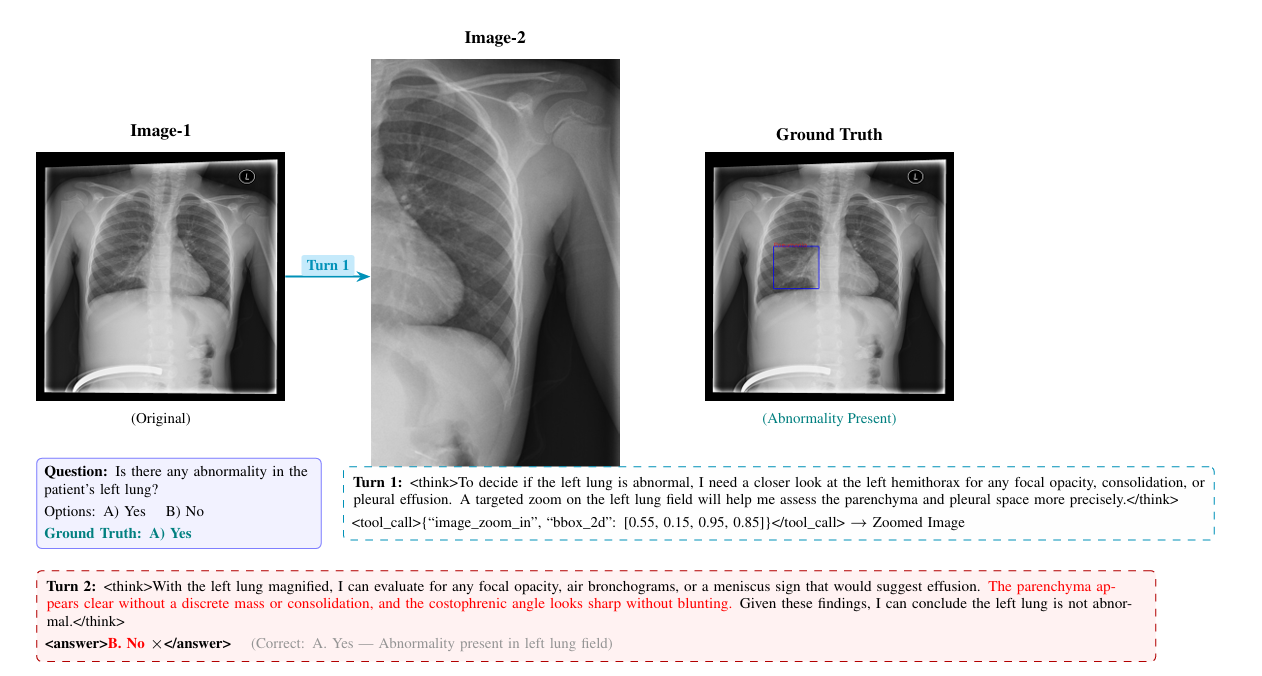
\includegraphics[width=\linewidth]{fig10a.png}
    \caption{Insufficient visual evidence: the agent correctly zooms into the left
     lung field but misses a subtle abnormality below the resolution of the tool
     at the applied scale.}
  \end{subfigure}\\[8pt]
  \begin{subfigure}{0.95\linewidth}
    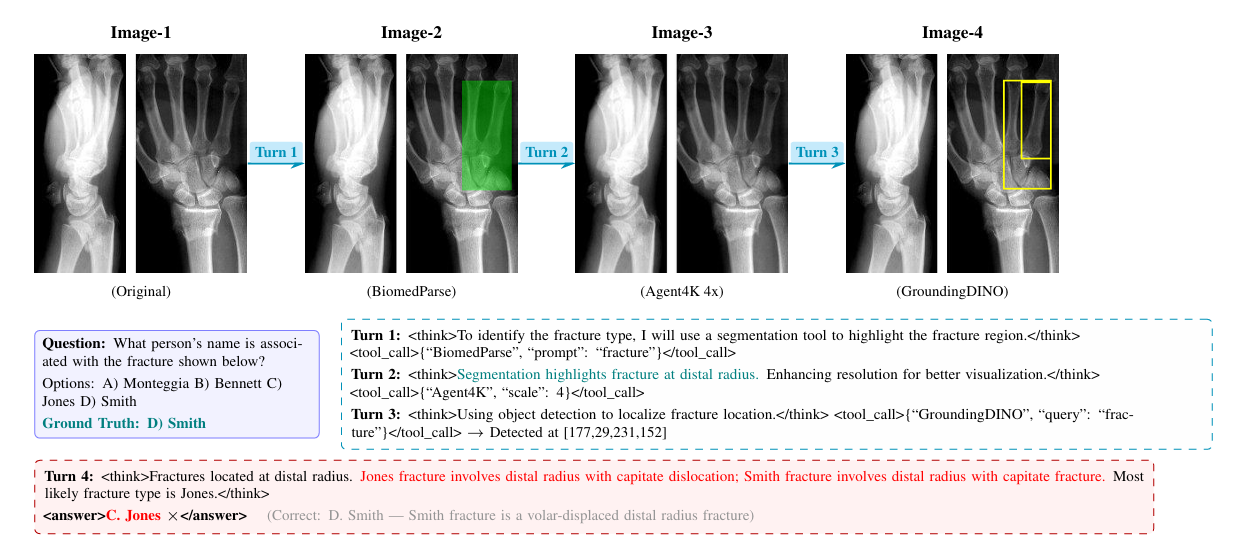
\includegraphics[width=\linewidth]{fig10b.png}
    \caption{Knowledge gap: all three tools locate the fracture correctly, but the
     agent confuses Jones and Smith fracture definitions and outputs the wrong
     eponym.}
  \end{subfigure}
  \caption{Two representative failure modes in MedVistaGym that highlight the limits
   of tool-augmented perception and the gap that domain knowledge must fill.
   Adapted from Lu et al.~\cite{medvistagym}.}
  \label{fig:10}
\end{figure}

\subsection{Promising Directions}

The convergence of point-and-click and tool invocation action spaces, whereby
IBISAgent's precise click space is combined with MedVistaGym's diverse set of tools,
represents a natural extension which is currently not accomplished by either system.
Process reward design needs additional exploration, particularly regarding the
overshoot penalty.

The use of a broader measure of rewards, considering both the validity of click
positions, improvements in quality margins, optimal stopping conditions, and the
suitability of the tools, will result in higher density training signals throughout
the process.

There is an immediate need for establishing benchmarking standards for the three
systems to be evaluated against each other.
Currently, IBISAgent~\cite{ibisagent}, MedVistaGym~\cite{medvistagym}, and
MedSAM-Agent~\cite{medsam_agent} are evaluated separately using different metrics,
making it impossible to compare them without recreating all three systems using the
same benchmarks.

% =============================================================
\section{Conclusion}
\label{sec:conclusion}
% =============================================================

This paper studies the three independently designed agentic systems for medical image
segmentation and reasoning---IBISAgent~\cite{ibisagent},
MedVistaGym/MedVista-R1~\cite{medvistagym}, and
MedSAM-Agent~\cite{medsam_agent}---using a common analytical framework considering
concept motivation, architectural design, training strategy, empirical validation, and
potential limitations.
As a group, the three systems show that viewing medical image analysis through the lens
of an iterative, feedback-guided decision-making task leads to significant and robust
performance gains on various benchmark datasets and imaging modalities.
The commonality of the two-stage SFT+RL training paradigm, visual observation encoding,
and multi-dimensional reward scheme in all three independent systems suggests that they
represent fundamental solutions to the core issues of clinical agentic AI, rather than
arbitrary engineering decisions.

On the other hand, the three systems differ from each other in several aspects due to
their different trade-offs between clinical realism and computational efficiency.
IBISAgent's exclusive use of point-and-click actions, along with a highly sophisticated
five-dimensional reward function, ensures superior segmentation performance but results
in lengthy average trajectories.
MedSAM-Agent's use of both bounding box and point selection mechanisms, paired with a
process-oriented reward function, achieves outstanding efficiency (2.11 average number
of turns) with decent accuracy.
The tool diversity mechanism adopted by MedVistaGym provides flexibility in multimodal
reasoning but requires a larger action space, which demands appropriate training
strategies.

The community is currently at a critical juncture.
The fundamental design principles for agentic medical image analysis have been
well-established.
Challenges that remain include extending agentic image analysis to 3D volume imaging,
grounding knowledge, prospective clinical validation, and standardized evaluation
criteria.

% =============================================================
\section*{References}
\addcontentsline{toc}{section}{References}
% =============================================================

\begin{thebibliography}{99}

\bibitem{ibisagent}
Y.~Jiang, Q.~Li, B.~Xu, H.~Sun, C.~Ding, J.~Dong, Y.~Cai, X.~Zhang, and J.~Yin,
``IBISAgent: Reinforcing Pixel-Level Visual Reasoning in MLLMs for Universal Biomedical
Object Referring and Segmentation,''
\textit{arXiv preprint arXiv:2601.03054v3}, Feb.~2026.

\bibitem{medvistagym}
M.~Lu, Y.~Lu, Y.~Zhuang, M.~Mullins, Y.~Xie, G.~Xiao, C.~Fleming, W.~Shi, and
X.~Wang,
``MedVistaGym: A Scalable Training Environment for Thinking with Medical Images via
Tool-Integrated Reinforcement Learning,''
\textit{arXiv preprint arXiv:2601.07107v1}, Jan.~2026.

\bibitem{medsam_agent}
S.~Liu, L.~Bao, Q.~Yang, W.~Geng, B.~Zheng, C.~Li, W.~Chen, H.~Peng, and Y.~Yuan,
``MedSAM-Agent: Empowering Interactive Medical Image Segmentation with Multi-turn
Agentic Reinforcement Learning,''
\textit{arXiv preprint arXiv:2602.03320v1}, Feb.~2026.

\bibitem{lisa}
X.~Lai, Z.~Tian, Y.~Chen, Y.~Li, Y.~Yuan, S.~Liu, and J.~Jia,
``LISA: Reasoning Segmentation via Large Language Model,''
in \textit{Proc.\ IEEE/CVF CVPR}, pp.~9579--9589, 2024.

\bibitem{unibiomed}
L.~Wu, Y.~Nie, S.~He, J.~Zhuang, L.~Luo, N.~Mahboobani, V.~Vardhanabhuti,
R.~C.~K.~Chan, Y.~Peng, P.~Rajpurkar et al.,
``UniBiomed: A Universal Foundation Model for Grounded Biomedical Image Interpretation,''
\textit{arXiv preprint arXiv:2504.21336}, 2025.

\bibitem{medsam2}
J.~Ma, Z.~Yang, S.~Kim, B.~Chen, M.~Baharoon, A.~Fallahpour, R.~Asakereh, H.~Lyu,
and B.~Wang,
``MedSAM2: Segment Anything in 3D Medical Images and Videos,''
\textit{arXiv preprint arXiv:2504.03600}, 2025.

\bibitem{mmedagent}
B.~Li, T.~Yan, Y.~Pan, J.~Luo, R.~Ji, J.~Ding, Z.~Xu, S.~Liu, H.~Dong, Z.~Lin, and
Y.~Wang,
``MMedAgent: Learning to Use Medical Tools with Multi-Modal Agent,''
\textit{arXiv preprint arXiv:2407.02483}, 2024.

\bibitem{unet}
O.~Ronneberger, P.~Fischer, and T.~Brox,
``U-Net: Convolutional Networks for Biomedical Image Segmentation,''
in \textit{Medical Image Computing and Computer-Assisted Intervention (MICCAI)},
pp.~234--241, 2015.

\bibitem{sam}
A.~Kirillov, E.~Mintun, N.~Ravi, H.~Mao, C.~Rolland, L.~Gustafson, T.~Xiao,
S.~Whitehead, A.~C.~Berg, W.-Y.~Lo, P.~Dollar, and R.~Girshick,
``Segment Anything,''
in \textit{Proc.\ IEEE/CVF CVPR}, pp.~4015--4026, 2023.

\bibitem{nnunet}
F.~Isensee, P.~F.~Jaeger, S.~A.~Kohl, J.~Petersen, and K.~H.~Maier-Hein,
``nnU-Net: A Self-Configuring Method for Deep Learning-Based Biomedical Image
Segmentation,''
\textit{Nature Methods}, vol.~18, no.~2, pp.~203--211, 2021.

\bibitem{medplib}
X.~Huang, L.~Shen, J.~Liu, F.~Shang, H.~Li, H.~Huang, and Y.~Yang,
``Towards a Multimodal Large Language Model with Pixel-Level Insight for Biomedicine,''
in \textit{Proc.\ AAAI Conf.\ Artificial Intelligence}, pp.~3779--3787, 2025.

\bibitem{citrusv}
G.~Wang, J.~Zhao, X.~Liu, Y.~Liu, X.~Cao, C.~Li, Z.~Liu, Q.~Sun, F.~Zhou, H.~Xing,
and Z.~Yang,
``Citrus-V: Advancing Medical Foundation Models with Unified Medical Image Grounding
for Clinical Reasoning,''
\textit{arXiv preprint arXiv:2509.19090}, 2025.

\bibitem{deepseekr1}
D.~Guo, D.~Yang, H.~Zhang, J.~Song, R.~Zhang, R.~Xu, Q.~Zhu, S.~Ma, P.~Wang, X.~Bi
et al.,
``DeepSeek-R1: Incentivizing Reasoning Capability in LLMs via Reinforcement Learning,''
\textit{arXiv preprint arXiv:2501.12948}, 2025.

\bibitem{vilam3}
V.~Nath, W.~Li, D.~Yang, A.~Myronenko, M.~Zheng, Y.~Lu, Z.~Liu, H.~Yin, Y.~Tang,
P.~Guo et al.,
``VILA-M3: Enhancing Vision-Language Models with Medical Expert Knowledge,''
in \textit{Proc.\ IEEE/CVF CVPR}, pp.~14788--14798, 2025.

\bibitem{aura}
N.~Fathi, A.~Kumar, and T.~Arbel,
``AURA: A Multi-Modal Medical Agent for Understanding, Reasoning and Annotation,''
\textit{arXiv preprint arXiv:2507.16940}, 2025.

\bibitem{qwen25vl}
S.~Bai, K.~Chen, X.~Liu, J.~Wang, W.~Ge, S.~Song, K.~Dang, P.~Wang, S.~Wang,
J.~Tang et al.,
``Qwen2.5-VL Technical Report,'' \textit{arXiv preprint arXiv:2502.13923}, 2025.

\bibitem{biomedparse}
T.~Zhao, Y.~Gu, J.~Yang, N.~Usuyama, H.~H.~Lee, S.~Kiblawi, T.~Naumann, J.~Gao,
A.~Crabtree, J.~Abel et al.,
``BioMedParse: A Biomedical Foundation Model for Image Parsing of Everything Everywhere
All at Once,'' \textit{arXiv preprint arXiv:2405.12971}, 2024.

\bibitem{deepinteractive}
N.~Xu, B.~Price, S.~Cohen, J.~Yang, and T.~S.~Huang,
``Deep Interactive Object Selection,''
in \textit{Proc.\ IEEE Conf.\ Computer Vision and Pattern Recognition}, pp.~373--381, 2016.

\bibitem{gemini25}
G.~Comanici, E.~Bieber, M.~Schaekermann et al.,
``Gemini 2.5: Pushing the Frontier with Advanced Reasoning, Multimodality, Long Context,
and Next Generation Agentic Capabilities,''
\textit{arXiv preprint arXiv:2507.06261}, 2025.

\bibitem{gpt5}
OpenAI, ``GPT-5 Chat,'' \url{https://chat.openai.com}, 2025. Accessed: 2025-09-17.

\bibitem{openreasonerzero}
J.~Hu, Y.~Zhang, Q.~Han, D.~Jiang, X.~Zhang, and H.-Y.~Shum,
``Open-Reasoner-Zero: An Open Source Approach to Scaling Up Reinforcement Learning on
the Base Model,'' \textit{arXiv preprint arXiv:2503.24290}, 2025.

\bibitem{pathvqa}
X.~He, Y.~Zhang, L.~Mou, E.~Xing, and P.~Xie,
``PathVQA: 30000+ Questions for Medical Visual Question Answering,''
\textit{arXiv preprint arXiv:2003.10286}, 2020.

\bibitem{slake}
B.~Liu, L.-M.~Zhan, L.~Xu, L.~Ma, Y.~Yang, and X.-M.~Wu,
``SLAKE: A Semantically-Labeled Knowledge-Enhanced Dataset for Medical Visual Question
Answering,'' in \textit{IEEE ISBI}, pp.~1650--1654, 2021.

\bibitem{vqarad}
J.~J.~Lau, S.~Gayen, A.~Ben~Abacha, and D.~Demner-Fushman,
``A Dataset of Clinically Generated Visual Questions and Answers about Radiology Images,''
\textit{Scientific Data}, vol.~5, no.~1, pp.~1--10, 2018.

\bibitem{imisnet}
J.~Cheng, B.~Fu, J.~Ye, G.~Wang, T.~Li, H.~Wang, R.~Li, H.~Yao, J.~Cheng, J.~Li
et al.,
``Interactive Medical Image Segmentation: A Benchmark Dataset and Baseline,''
in \textit{Proc.\ IEEE/CVF CVPR}, pp.~20841--20851, 2025.

\bibitem{qwen3vl}
S.~Bai, Y.~Cai, R.~Chen et al.,
``Qwen3-VL Technical Report,'' \textit{arXiv preprint arXiv:2511.21631}, 2025.

\bibitem{segr1}
Z.~You and Z.~Wu,
``Seg-R1: Segmentation Can Be Surprisingly Simple with Reinforcement Learning,''
\textit{arXiv preprint arXiv:2506.22624}, 2025.

\end{thebibliography}

\end{document}